\documentclass[letterpaper,11pt]{article}

% Packages
\usepackage[utf8]{inputenc}
\usepackage{geometry}
\usepackage{titlesec}
\usepackage{enumitem}
\usepackage{hyperref}
\usepackage{xcolor}
\usepackage{amsmath}
\usepackage{amssymb}
\usepackage{fancyhdr}
\usepackage{graphicx}
\usepackage{float}
\usepackage{booktabs}
\usepackage{tabularx}
\usepackage{listings}
\usepackage{setspace}
\usepackage[toc]{appendix}
\singlespacing

% Page Setup
\geometry{left=2.5cm, right=2.5cm, top=2.5cm, bottom=2.5cm}
\setlength{\headheight}{14pt}
\pagestyle{fancy}
\fancyhf{}
\rhead{\textbf{Final Report}}
\lhead{01 - CP683-BF - 4/2026}
\cfoot{\thepage}

% Custom Colors
\definecolor{primary}{RGB}{0, 51, 102}
\definecolor{accent}{RGB}{204, 0, 0}

% Title Format
\titleformat{\section}
{\normalfont\Large\bfseries\color{primary}}{\thesection}{1em}{}

\titleformat{\subsection}
{\normalfont\large\bfseries\color{primary}}{\thesubsection}{1em}{}

% Code listing style
\lstdefinestyle{code}{
    backgroundcolor=\color{gray!8},
    basicstyle=\ttfamily\small,
    keywordstyle=\color{blue},
    commentstyle=\color{gray},
    stringstyle=\color{teal},
    breaklines=true,
    frame=single,
    numbers=left,
    numberstyle=\tiny\color{gray},
    tabsize=2
}
\lstset{style=code}

% Metadata
\title{\textbf{AIVS: Anonymous Identification Verification System}\\Based on Ring Signatures with Isolated Smart Card Hardware}
\author{
\textit{Dinh Anh Khoa Nguyen - 245849840 - nguy9840@mylaurier.ca}\\
\textit{Jiangtao Wang - 245823800 - Wang2370@mylaurier.ca}\\
\textit{Leila Chen - 245850620 - chen5062@mylaurier.ca}\\
\textit{Yuyang Wu - 245817310 - wuxx7310@mylaurier.ca}\\
}
\date{April 2026}

\begin{document}

\maketitle
\thispagestyle{empty}

\begin{abstract}
    This report outlines the engineering implementation of a privacy-preserving messaging platform that decouples message integrity from identity revelation. Leveraging Yubikey hardware PRF and nested Ring Signatures, the system allows users to send undeniable, tamper-proof messages anonymously, with the exclusive capability to retroactively prove authorship. The project adopts an Agile methodology, utilizing React/TypeScript for the frontend and Node.js for the backend.
\end{abstract}
\newpage

\tableofcontents
\newpage

% ============================================================
\section{Introduction}

\subsection{Motivation and Problem Statement}
In current cryptographic systems, users typically face a binary choice:
\begin{enumerate}
    \item \textbf{Signed Messages:} Authenticity is guaranteed, but privacy is compromised immediately (e.g., PGP).
    \item \textbf{Anonymous Messages:} Privacy is maintained, but credibility is low, and the author cannot later claim credit or reputation for the content (e.g., Tor-based drops).
\end{enumerate}
There is a lack of infrastructure that supports \textit{conditional anonymity}. Where a user can speak freely now and prove they spoke later, without relying on a trusted third party.

\subsection{Project Objectives}
\begin{itemize}
    \item \textbf{Objective A:} Anonymous message dispatching where the sender is mathematically hidden among a set of 7 decoys (1-of-8 Ring Signature).
    \item \textbf{Objective B:} Integrity verification by the recipient without identity knowledge.
    \item \textbf{Objective C:} A ``Challenge-Response'' flow where the sender can prove authorship by unlocking a cryptographic proof using their physical Yubikey.
\end{itemize}

\subsection{Scope and Limitations}
AIVS is a research prototype that is used to demonstrate the combination of cryptography with a two-party messaging system to present conditional anonymity. The system consists of anonymous message, verification, and authorship proof via a hardware based Yubikey. All important operations are performed on the client browser side, while the backend server serves as a relay and a storage service, without knowing the identity of users.
As a prototype, there are several limitations in the current implementation:
\begin{itemize}
    \item \textbf{Anonymity Set Size:} The ring of public keys is fixed at 1-of-8 (one real public key and seven generated decoy ones). This is sufficient for a prototype, but is not suitable for larger schemes, which provide stronger anonymity guaranties and are more appropriate for production systems.
    \item \textbf{Hardware Dependency:} The system specifically requires a physical hardware device named Yubikey with PRF extension support. Environments with different hardware cannot participate in the process.
    \item \textbf{Prototype Scope:} The implementation is not designed for production use. Such factors as: Scalability, multi-device support and account recovery are not in scope.
\end{itemize}

% ============================================================
\section{Background and Related Work}
\subsection{Ring Signatures --- Theory and Prior Work}

Rivest, Shamir, and Tauman have introduced Ring signatures which can provide a mechanism for anonymous authentication by leveraging a predefined set of public keys. This mechanism relies on a signature being generated by a signer on behalf of a group and can be verified to confirm that one of the group members signed the message without revealing the exact signer.
Differing from group signature schemes, a trusted setup phase, a group manager, or a revocation mechanism are not required for ring signatures. So, by selecting a set of public keys, the ring can be independently constructed by the signer. This makes the scheme particularly suitable for decentralized settings.
Linkable Ring Signature (LRS) is an important extension of this concept. In LRS schemes, each signature includes a linking tag which is often known as a key image. This tag is generated based on the signer's secret key and the public key. The purpose of this tag is to link different signatures produced by the same signer and to keep the signer’s identity secret. Because of this feature, this schema is widely used in cryptocurrency systems, as it can prevent double spending and preserve anonymity.
In this project, this LRS is used in a different context which is establishing a verifiable relationship between two signatures generated from the same one-time key. As a result of this mechanism, a controlled disclosure workflow is generated and this workflow can demonstrate authorship by revealing additional information and preserve anonymity by default.

\subsection{Hardware Security Tokens and WebAuthn PRF}

Secret keys management is also an important aspect in the context of security of cryptographic systems. In many browser-based applications, key material is handled in software, but this may enhance the risk of cross-site scripting (XSS) and cause a compromised execution environment.
The FIDO2/WebAuthn standard introduces a model to allow cryptographic operations to be performed by external authenticators, such as hardware security tokens. In this model, the host application cannot directly access the private keys which are generated and stored within the authenticator.
A recent extension to WebAuthn is the PRF (Pseudo-Random Function) extension. In this extension, by giving an input, an output would be generated based on a credential-bound secret and it is accessible to the application. The authenticator can return the PRF output while keeping the underlying secret. As a result, applications can derive high-entropy values tied to the authenticator.
In this project, PRF outputs are used as part of the key derivation process for one-time signing keys. And they also are used for deriving symmetric keys used in proof encryption. This design creates a connection between critical cryptographic operations and the possession of a hardware authenticator, so that the reliance on software-managed long-term secrets in the browser environment can be significantly reduced.

% ============================================================
\section{System Design}

\subsection{Architecture Overview}
The system follows a \textbf{Thick Client, Thin Server} architecture. The server acts purely as a bulletin board and relay, possessing zero knowledge of user identities or private keys, and is explicitly excluded from the trusted computing base.

\subsection{Security Model and Threat Model}
\begin{itemize}
    \item \textbf{Key Derivation:} The OTK is derived with the participation of the Yubikey, ensuring it cannot be predicted or extracted.
    \item \textbf{Anonymity Set:} 1 real signer + 7 random decoys = 8 total keys. Probability of guessing the signer is $1/8$ per message (statistically negligible for identification).
    \item \textbf{Forward Secrecy:} Compromise of the Yubikey allows decryption of past Proofs but does not reveal the identity of past messages \textit{unless} the attacker actively performs the decryption and linking.
\end{itemize}

\subsection{Cryptographic Construction}
\begin{enumerate}
    \item \textbf{Setup:} Generate One-Time Key ($OTK$) via Yubikey. Generate 7 Fake Keys ($FK_{1...7}$).
    \item \textbf{Inner Layer (The Proof):}
          $$ Sig_{inner} = RingSign(Message, \{OTK, FK_{1...7}\}) $$
          $$ Key_{proof} = KDF(PRF_{Yubikey}(Hash(OTK))) $$
          $$ Proof = Encrypt_{AES-GCM}(Sig_{inner}, Key_{proof}) $$
          where the hash of the $OTK$ is used as a salt to bind the proof key to the one-time signing key.
    \item \textbf{Outer Layer (The Transmission):}
          $$ Sig_{outer} = RingSign(Message || Hash(Sig_{inner}), \{OTK, FK_{1...7}\}) $$
    \item \textbf{Verification:} Upon decryption, the Linkable Tag of $Sig_{inner}$ must equal the Linkable Tag of $Sig_{outer}$.
\end{enumerate}

\subsection{Component Diagram}
\begin{verbatim}
[Client A (Sender)]          [Server (Node.js)]          [Client B (Recipient)]
       |                            |                            |
   (Yubikey)                        |                            |
       | -- Gen OTK & Sig -->       |                            |
       | -- POST Message --->       |                            |
       |                            | -- Store Message -->       |
       |                            |                            |
       |                            | -- WS / Push Event -->     |
       |                            |                            |
       |                            |             (Verify Outer Sig locally)
       |                            |                            |
   (Challenge) <------------------  | <----- Request Proof ----- |
       |                            |                            |
   (Decrypt Proof)                  |                            |
       | -- Send Decrypted Sig ->   |                            |
       |                            | -- Forward Sig ----------> |
       |                            |                            |
       |                            |             (Verify Inner Sig & Link)
\end{verbatim}

\subsection{Data Flow Diagram}
\begin{enumerate}
    \item \textbf{Registration:} None required for the messaging protocol itself (stateless). Optional username registration maps public handles to WebAuthn Credential IDs for routing.
    \item \textbf{Signing:} All cryptographic operations occur in the browser memory. The Yubikey is accessed via \texttt{navigator.credentials.get(\char123 prf: ... \char125)}.
\end{enumerate}

\subsection{Database Schema}
The database is implemented in PostgreSQL and consists of five tables. The server stores only public key in binary data type and metadata for message routing and username verification.

\begin{figure}[H]
    \centering
    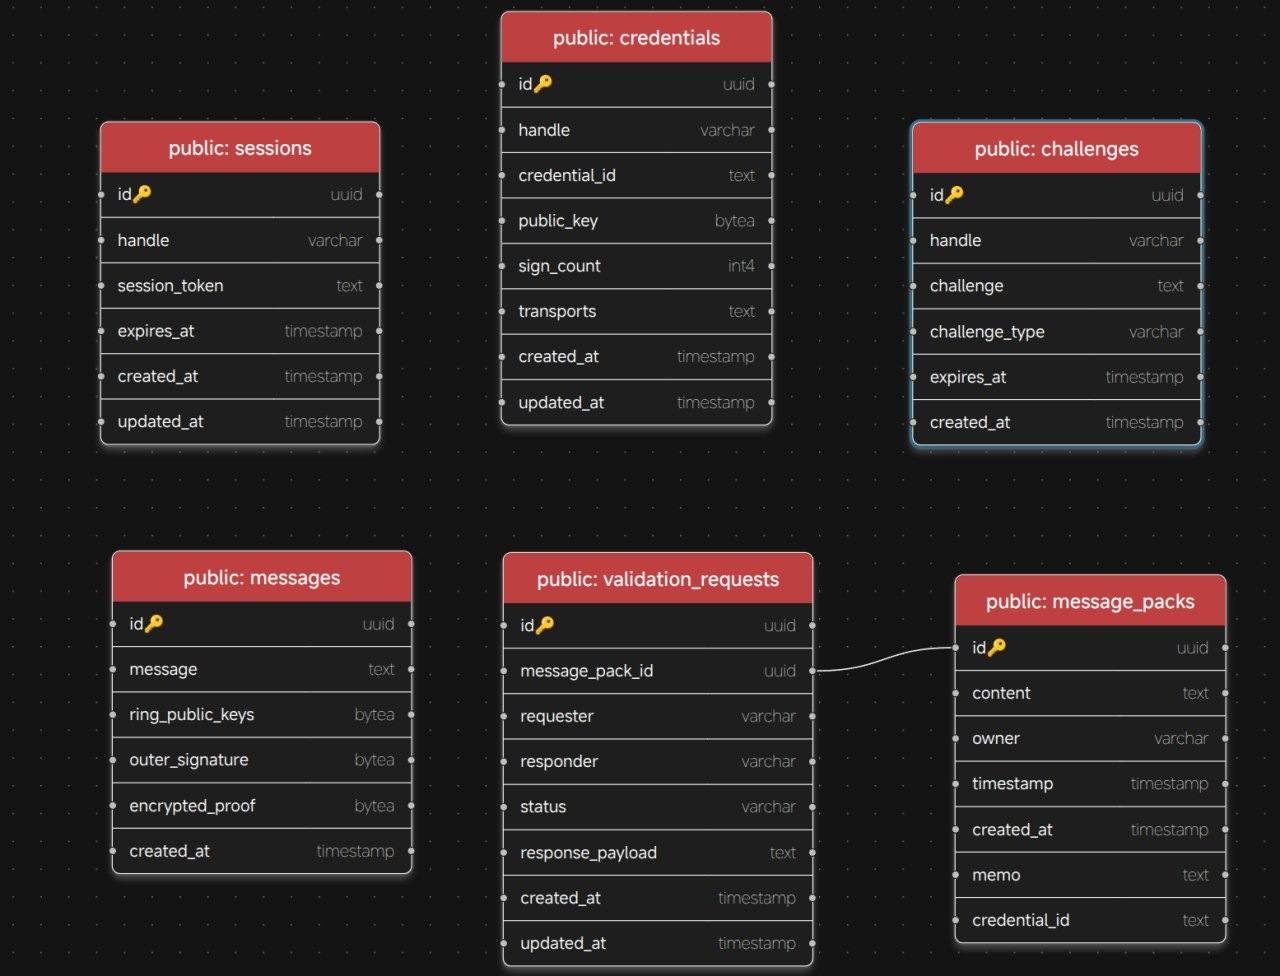
\includegraphics[width=0.95\textwidth]{database-schema.jpg}
    \caption{Database schema diagram showing the relationships between schemas, Powered by Gemini.}
\end{figure}

% ============================================================
\section{Implementation}

\subsection{Technology Stack}
\begin{itemize}
    \item \textbf{Frontend:} React, TypeScript.
    \item \textbf{Cryptography (Client):} WebAuthn API (PRF extension), Elliptic Curve Library (e.g., \texttt{elliptic} or WASM-based Rust bindings) for Ring Signatures.
    \item \textbf{Backend:} Node.js (Express/NestJS).
    \item \textbf{Database:} PostgreSQL (Stores only blobs: Message, Public Keys Ring, Signature, Encrypted Proof).
\end{itemize}

\subsection{Cryptography Module}

This module implements the core cryptographic operations. The core functions of this module are implements of a LRS based on Ristretto255 and Ed25519 curves. We can divided the module into four main components: core cryptographic implementation, key management, serialization tools and utility Functions.

\paragraph{Core Cryptographic Implementation} The core functionality of the part revolves around LRS, which allows a user to sign a message anonymously on behalf of a group (ring) while providing a way to "link" signatures if the same member signs multiple times.

\begin{itemize}
    \item \textbf{Data Structures}: It defines \texttt{LRSSignature} and \texttt{LRSSignatureRaw} interfaces to store signature components: \texttt{c0} (initial hash), \texttt{r} (responses), \texttt{I} (linkability tag/key image), and \texttt{ring} (public keys).
    \item \textbf{Signature Generation}:
          \begin{itemize}
              \item \texttt{generateLRS}: Generates a signature given a message, a set of public keys, the signer's index, and the signer's private key.
              \item \texttt{generateLRSWithoutFakeKeys}: A helper that automatically generates random ``fake'' keys to fill the ring, simplifying the signing process for a single user.
          \end{itemize}
    \item \textbf{Verification}:
          \begin{itemize}
              \item \texttt{verifyLRS}: Validates the signature by reconstructing the hash chain across the ring and checking if it matches the provided \texttt{c0}.
          \end{itemize}
\end{itemize}

\paragraph{Key Management} This part provides methods for managing cryptographic keys using the Ristretto255 curve:

\begin{itemize}
    \item \textbf{\texttt{generateKeyPair}}: Creates a public/private key pair, optionally from a provided seed for deterministic generation.
    \item \textbf{\texttt{validatePublicKey}}: Verifies that a specific public key corresponds to a given private key.
\end{itemize}

\paragraph{Serialization Tools and Utility Functions}

To facilitate data transmission and storage, the part includes utilities to convert signature objects to and from byte formats. Including \texttt{LRSToBytes}, \texttt{bytesToLRS}, \texttt{bytesToRawLRS}, textbf{Hashing}, \textbf{Data Conversion} and \textbf{Comparison}.

\paragraph{Conclusion} In conclusion, the cryptography module is designed to be efficient and secure, ensuring that all operations are performed locally on the client side with the assistance of the Yubikey, while the server remains a passive relay that handles only opaque data blobs.

\subsection{YubiKey Integration via WebAuthn PRF}

This component handles the interaction with the YubiKey hardware token using the WebAuthn API, specifically leveraging the PRF extension to derive one-time keys for signing and encryption. This is the main component that ensures the security of the key material by keeping it within the hardware boundary. For its implementation, it can be divided into two different parts:

\paragraph{WebAuthn and Hardware Key Derivation}
The system utilizes the \textbf{WebAuthn PRF \\ (Pseudo-Random Function) extension} to securely derive cryptographic keys from the user's hardware authenticator (e.g., TouchID, FaceID, or YubiKey) rather than storing private keys in plain text.

\paragraph{Cryptographic MessagePack Processing}
This is the core privacy logic that implements Linkable Ring Signatures (LRS) to ensure anonymity and verifiability.

\subsection{Backend API}
The backend API is implemented as a Noje.js RESTful API consisted of 4 services:
WebAuthn service, Message pack service, Validation request service and an authentication middleware. The middleware is used to validate session tokens between API calls of message pack service and validation request services.

\subsubsection*{WebAuthn Service}
Handles YubiKey credential registration and generates session token for authentication.

\begin{itemize}
    \item \texttt{POST /register/challenge} --- Create a registration challenge for a new credential.
    \item \texttt{POST /register/publickey} --- Final step of the registration process by storing the authenticator public key.
    \item \texttt{POST /auth/challenge} --- Create an authentication challenge for login.
    \item \texttt{POST /auth/session} --- Verify the challenge along with the response and generate a session token.
    \item \texttt{GET /session} --- Returns the current authenticated session (auth required, use to test the authentication).
\end{itemize}

\subsubsection*{Message Pack Service}
Handles creation, retrieval, and ownership transfer of message packs.

\begin{itemize}
    \item \texttt{POST /message} --- Create a new message pack.
    \item \texttt{GET /message/by\_id/:id} --- Retrieve a message pack by UUID.
    \item \texttt{GET /message/list/by\_username/:username} --- List all message packs owned by a given handle.
    \item \texttt{PUT /message/by\_id/:id/owner} --- Transfer ownership of a message pack to another handle.
\end{itemize}

\subsubsection*{Validation Request Service}
Manages the challenge-response flow between 2 users for authorship verification.

\begin{itemize}
    \item \texttt{POST /validation-requests} --- Create a new validation request for a message pack.
    \item \texttt{GET /validation-requests/sent} --- List validation requests created by the current user.
    \item \texttt{GET /validation-requests/received} --- List validation requests assigned to the current user.
    \item \texttt{PUT /:id/respond} --- User submits the decrypted signature as evidence.
    \item \texttt{PUT /:id/result} --- User finalizes the validation request after verifying the evidence.
\end{itemize}

\subsubsection*{Authentication Middleware}
\begin{itemize}
    \item \textbf{Auth middleware} --- Validates the session token on each protected API request.
\end{itemize}

\subsection{Frontend UI}

The frontend project is structured as a Single-Page Application (SPA). The overall architecture can be summarized as: \textbf{Single-Page Entry + Authentication Gateway + Signing Workbench + Data Request Utility Layer}.
In terms of implementation style, it follows a React functional layered architecture, with the core business logic centered around WebAuthn authentication and cryptographic signing workflows.

\paragraph{Application Entry Layer}
\begin{itemize}[leftmargin=2em]
    \item \texttt{index.html}: Provides the \texttt{root} container and loads \texttt{/src/main.tsx}.
    \item \texttt{src/main.tsx}: Creates the React Root, injects \texttt{StrictMode}, and mounts the application.
\end{itemize}

\paragraph{Application Shell Layer}
\begin{itemize}[leftmargin=2em]
    \item \texttt{src/App.tsx}: The application shell component; currently lightweight, primarily responsible for rendering the login wrapper component.
    \item \texttt{src/App.css}: Global base styles (root container and heading styles).
\end{itemize}

\paragraph{Authentication and Session Layer}
\begin{itemize}[leftmargin=2em]
    \item \texttt{src/login.tsx}: The primary business entry point, responsible for fetching registration/login challenges, invoking WebAuthn, managing session tokens, and switching the UI post-login.
    \item Supports Message Pack file imports, serving as the bridge between the authentication domain and the business domain.
\end{itemize}

\paragraph{Business Feature Layer (Signing and Verification)}
\begin{itemize}[leftmargin=2em]
    \item \texttt{src/Sign.tsx}: An aggregation layer for the signing workbench, using a collapse panel to organize features:
          \begin{itemize}[leftmargin=2em]
              \item Create new signed messages
              \item Message Pack list
              \item Received/Sent verification request lists
          \end{itemize}
    \item \texttt{src/Message.tsx}: List details and operations layer, responsible for:
          \begin{itemize}[leftmargin=2em]
              \item Message Pack detail display and local validation
              \item File export
              \item Ownership transfer
              \item Sending identity confirmation requests
              \item Request verification/rejection workflows
          \end{itemize}
\end{itemize}

\paragraph{Domain and Infrastructure Layer}
\begin{itemize}[leftmargin=2em]
    \item \texttt{src/utils.ts}: The core utility layer, handling API communication, cryptographic process encapsulation, authentication header assembly, and type definitions.
    \item This file also provides Message Pack construction and validation logic, serving as a critical dependency for upper-layer components.
\end{itemize}

\paragraph{Reserved Layer}
\begin{itemize}[leftmargin=2em]
    \item \texttt{src/constants.ts}: Currently empty; can serve as a unified entry point for constants in the future.
    \item \texttt{src/assets/}: Currently stores static resources (e.g., \texttt{react.svg}).
\end{itemize}

\paragraph{Rendering Flow} This application rendered in this flow: \\
\texttt{index.html} $\rightarrow$ \texttt{main.tsx} $\rightarrow$ \texttt{App.tsx} $\rightarrow$ \texttt{login.tsx} $\rightarrow$ \texttt{Sign.tsx} $\rightarrow$ \texttt{Message.tsx}

\paragraph{State Flow}
The project relies primarily on React local state (\texttt{useState} or \texttt{useEffect} \\ or \texttt{useCallback}); no global state management library is introduced.
Session state is persisted via \texttt{sessionStorage}, and user state is restored via session APIs after a refresh.

\paragraph{Data Flow}
UI components call functions in \texttt{src/utils.ts}, and the utility layer performs unified access to the backend \texttt{/api}.
In the development environment, Vite proxies and forwards requests to local backend services.

\paragraph{Dependency Boundaries}
\begin{itemize}[leftmargin=2em]
    \item UI and Interaction: React + Ant Design
    \item Shared Types and Cryptography: \texttt{@repo/shared}
    \item Build and Development: Vite + TypeScript + ESLint
\end{itemize}

\paragraph{Strengths}
\begin{itemize}[leftmargin=2em]
    \item Clear Layering: Distinct boundaries between page orchestration and infrastructure capabilities.
    \item Comprehensive Typing: Request/response types are centrally defined in the utility layer.
    \item Complete Business Loop: Covers core processes including login, signing, requesting, verification, and import/export.
\end{itemize}

\subsection{End-to-End Flow: Alice \texorpdfstring{$\rightarrow$}{--->} Bob \texorpdfstring{$\rightarrow$}{--->} Reveal}
The system involves three primary roles: the Sender, the Recipient, and a Backend Server, with a YubiKey hardware token participating in cryptographic operations. Both the Sender and the Recipient interact with the system through a web browser, while the backend server functions solely as a message relay and storage service.

All cryptographic operations are performed locally on the client side with the assistance of the YubiKey. The server does not generate, store, or process private keys, and only handles opaque data blobs, including messages, signatures, and encrypted proofs. The YubiKey is used to provide hardware-bound PRF outputs that participate in one-time key derivation and proof encryption, without exposing secret material to the browser or operating system.

The system does not maintain a global signing key registry. Each message is associated with a freshly derived one-time key, and no signing keys are reused across messages.

During message transmission, the Sender composes a message using a browser-based client with a connected YubiKey. A one-time key is derived with the participation of the YubiKey and used, together with a fixed set of randomly generated decoy keys, to construct a ring signature over the message. To support future authorship verification, an additional inner ring signature is generated and encrypted as a proof using a symmetric key derived from the YubiKey PRF output. An outer ring signature is then computed over the message concatenated with the hash of the encrypted proof. The message, outer signature, and encrypted proof are transmitted to the Recipient via the backend server.

Upon receipt, the Recipient verifies the outer ring signature to confirm message integrity and authenticity, while the Sender's identity remains hidden within the anonymity set. The encrypted proof is not required for this initial verification.

If identity verification is later requested, the Recipient sends the original message, signature, and encrypted proof to the claimed Sender. Using the same YubiKey, the Sender derives the corresponding decryption key and decrypts the proof to reveal the inner ring signature. The decrypted signature is returned to the Recipient, who verifies its validity and linkability against the original message and signature to confirm authorship.

% ============================================================
\section{Evaluation}

\subsection{Functional Testing}
Functional testing was conducted to verify that the prototype supports the intended end-to-end workflow, including authentication, anonymous message creation, message-pack management, and authorship confirmation. Rather than assessing user interface quality in isolation, this evaluation focused on whether the frontend, backend, and client-side cryptographic components operated consistently as an integrated system.

The first group of tests focused on the WebAuthn-based login flow. A user was able to initiate registration or authentication challenges from the browser, complete credential operations with the hardware token, and obtain a valid session for subsequent requests. After successful login, the client correctly restored the authenticated state and exposed the corresponding user functions, indicating that challenge handling, session issuance, and session recovery were workflow-level functional successes.

\begin{figure}[H]
    \centering
    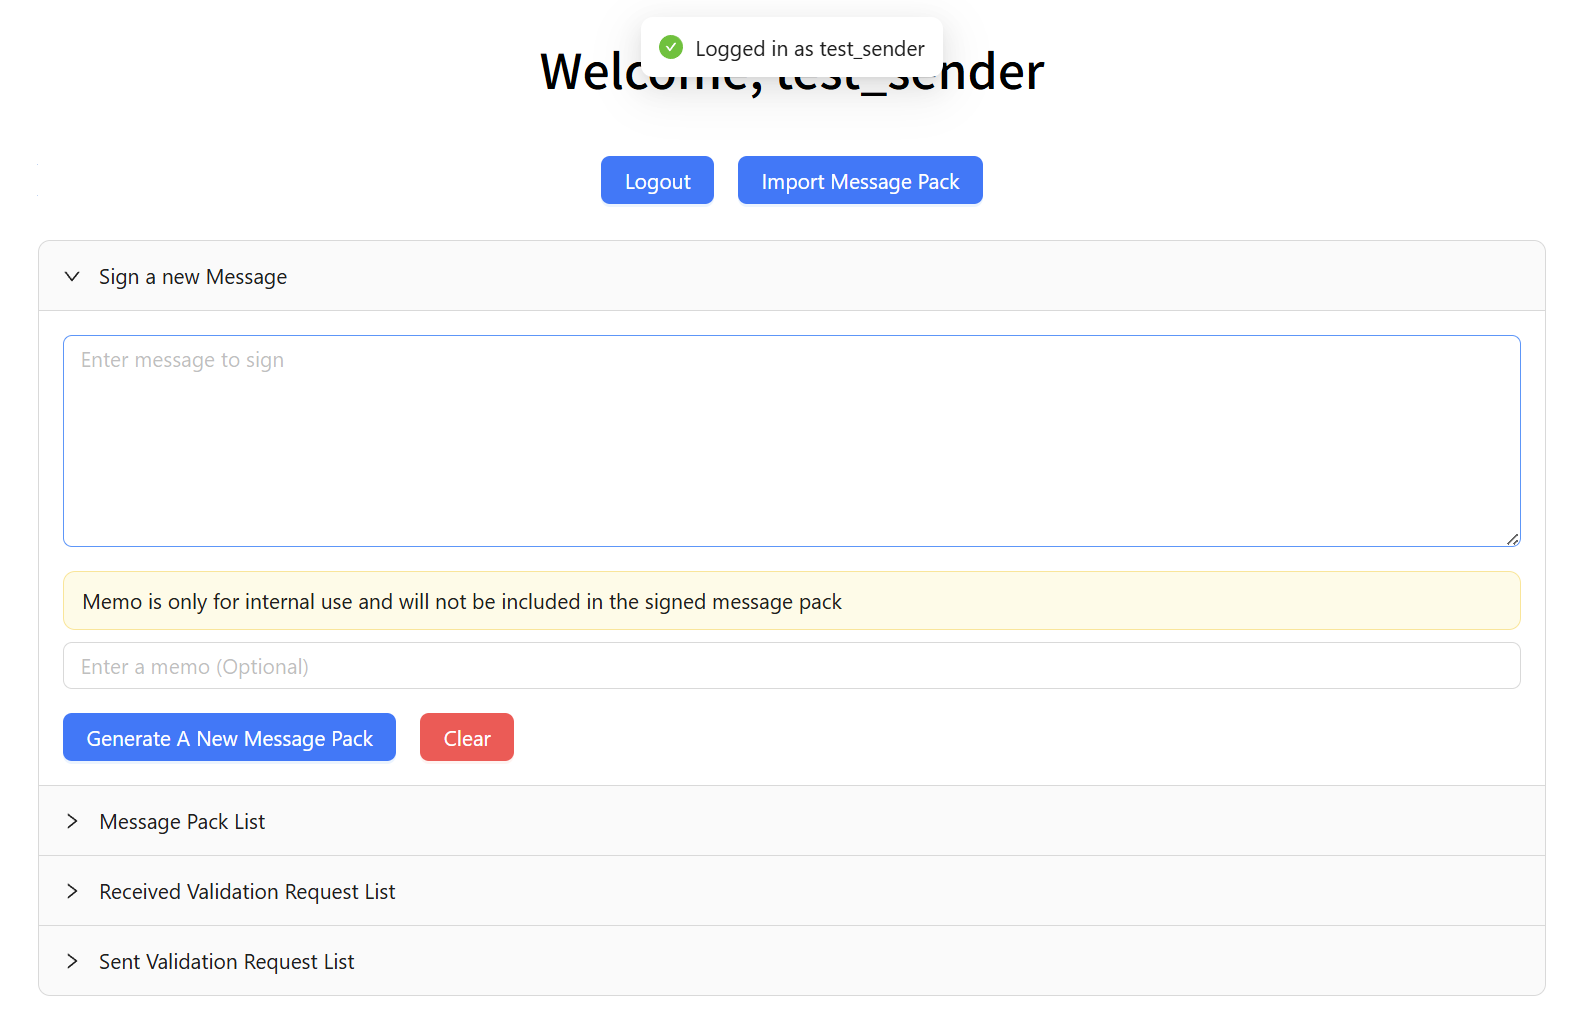
\includegraphics[width=0.70\textwidth]{functional-login-success.png}
    \caption{Authenticated user interface after successful login and session establishment.}
\end{figure}

The second group of tests examined anonymous message-pack generation and storage. After authentication, the client successfully derived a one-time key with the participation of the YubiKey PRF, generated the corresponding ring-signature-based message pack locally, and submitted the serialized result to the backend. The stored message pack could then be retrieved and displayed in the message list, confirming that local cryptographic generation, backend persistence, and frontend rendering were correctly connected.

\begin{figure}[H]
    \centering
    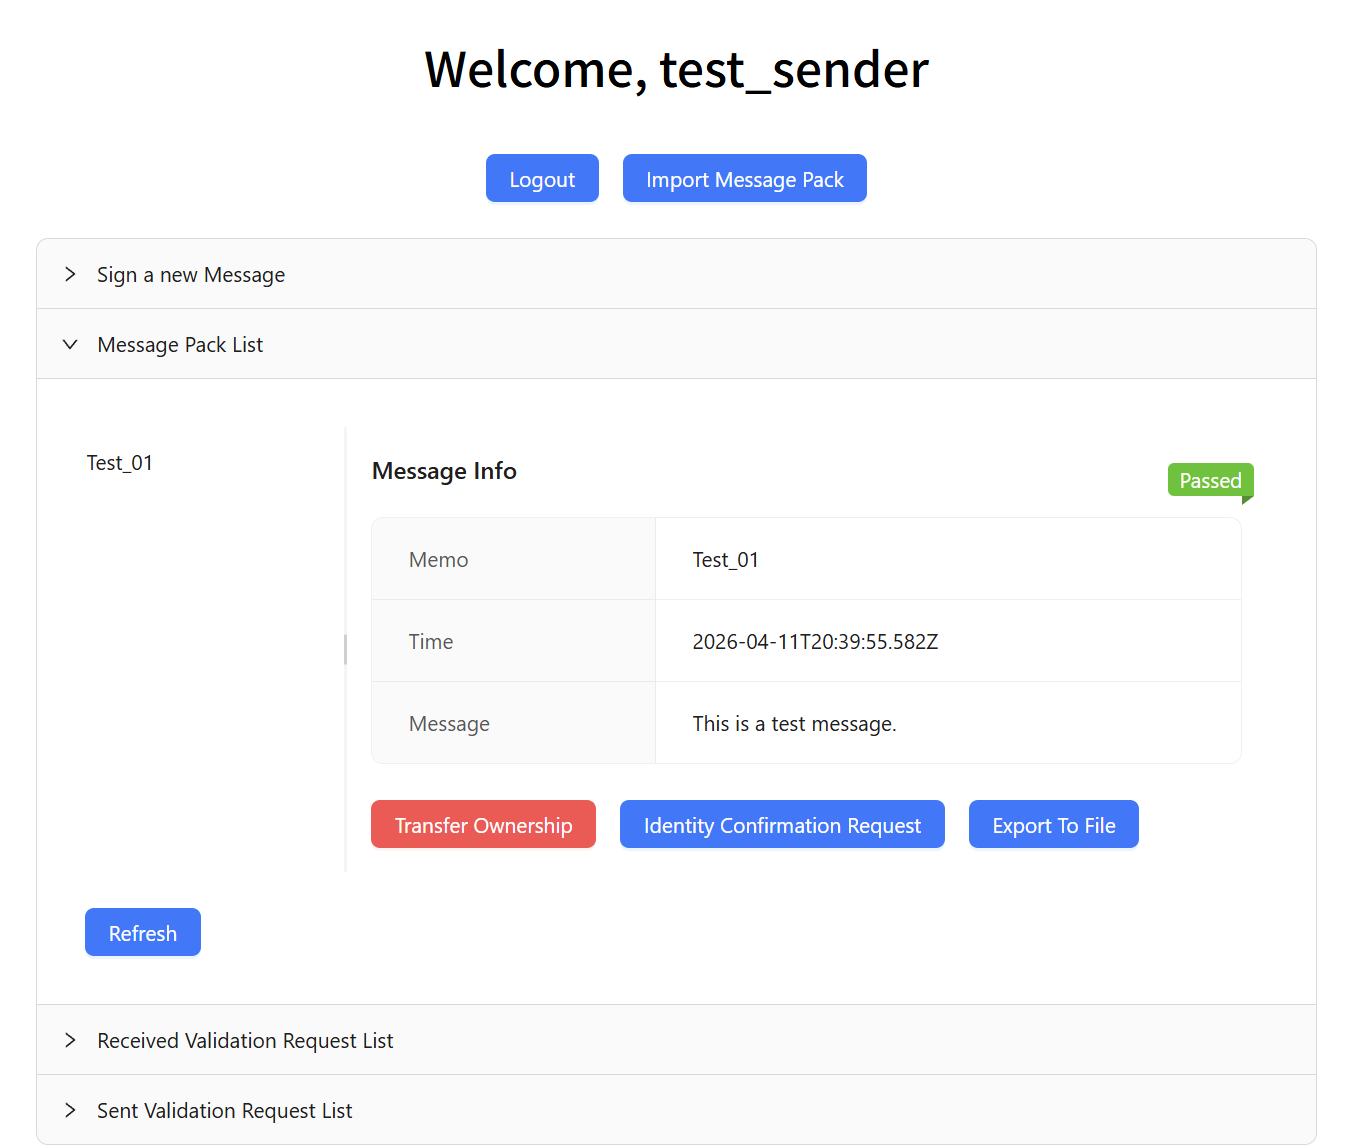
\includegraphics[width=0.65\textwidth]{functional-message-pack.png}
    \caption{Stored message pack displayed in the list with management actions.}
\end{figure}

Additional tests covered message-pack management and the authorship confirmation workflow. A user could export a stored message pack, transfer its ownership to another user, and observe the updated ownership state after refreshing the list. Furthermore, a recipient could initiate a validation request, the claimed sender could respond with a proof derived from the original credential, and the requester could obtain a final validation status. These results indicate that the prototype already supports the complete functional loop from anonymous message creation to later identity revelation.

\begin{figure}[H]
    \centering
    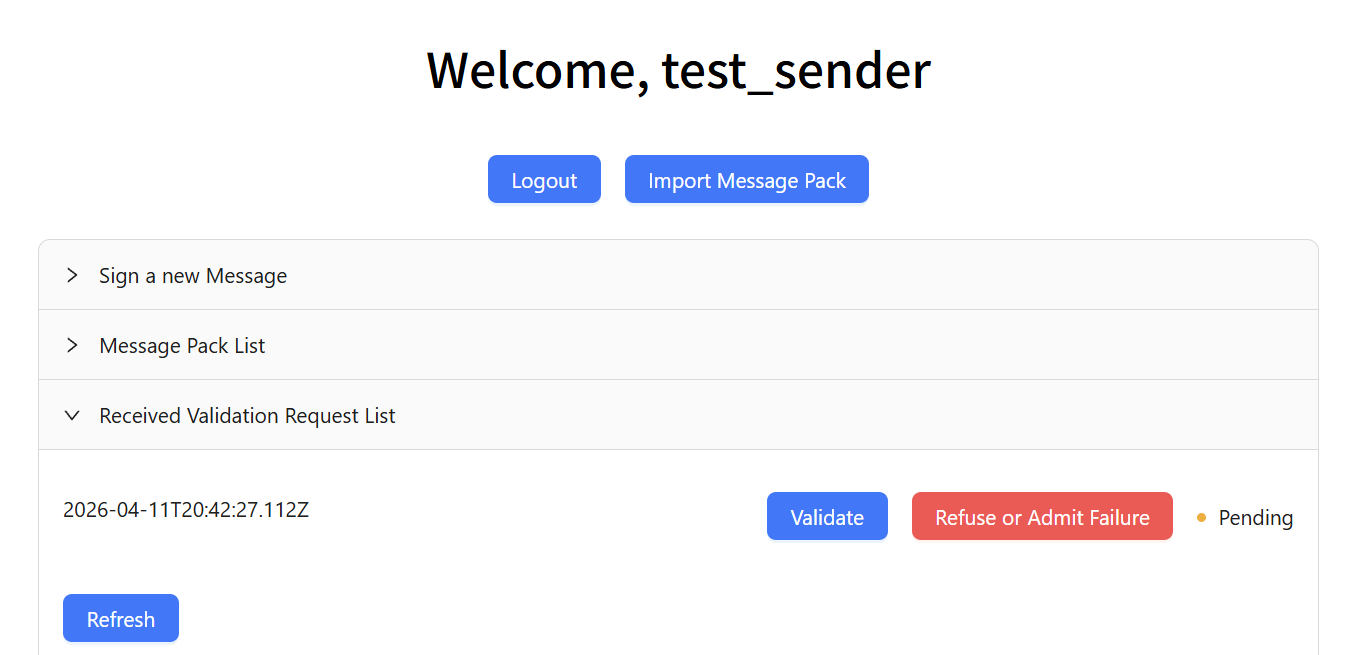
\includegraphics[width=0.65\textwidth]{functional-validation-received.png}
    \caption{Received validation request shown in the pending state before proof handling.}
\end{figure}

\begin{figure}[H]
    \centering
    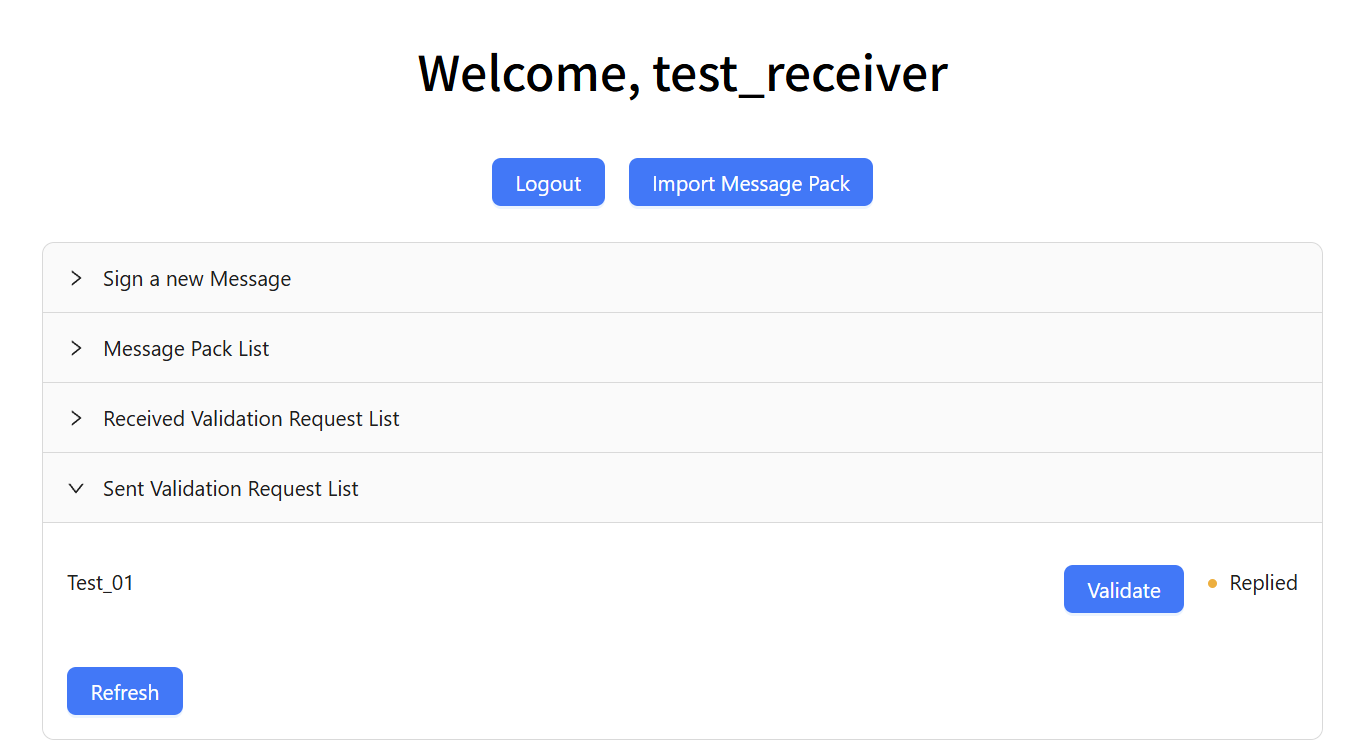
\includegraphics[width=0.65\textwidth]{functional-validation-replied.png}
    \caption{Sent validation request shown after the responder has returned a proof.}
\end{figure}

\subsection{Security Analysis}
The security properties of the prototype are primarily derived from the combination of client-side cryptographic execution, hardware-assisted key derivation, and the two-layer ring-signature construction. Instead of directly signing messages with a long-term identity key, the system derives a one-time key with the participation of the YubiKey through the WebAuthn PRF extension. As a result, message authenticity can be established without introducing a direct and persistent link between signed content and the user's long-term identity.

First, the system supports anonymous authenticity. The outer ring signature allows a recipient to verify that a message was produced by a valid member of the ring without revealing which member actually signed it. Because each message is associated with a freshly derived one-time key and a set of decoy public keys, signatures are not directly tied to a stable long-term identity.

Second, the prototype supports controlled authorship revelation. In addition to the outer signature, the sender generates an inner ring signature and protects it as an encrypted proof derived from the same hardware-backed credential. This allows the sender to later provide additional cryptographic evidence and confirm authorship when needed.

Third, the backend does not store private signing material and does not perform the cryptographic operations required to generate or reveal proofs. Its role is limited to challenge management, session handling, message-pack storage, and validation-request coordination. As a result, the server is not required to act as a trusted identity escrow for the messaging workflow.

Overall, the prototype demonstrates that anonymous transmission, integrity verification, and later authorship confirmation can coexist within one browser-based workflow.

\subsection{Performance Analysis}
Functional testing and backend API timing observations were conducted through the online test environment at \texttt{https://cp683.ryonanamizu.com/}. The system was accessed through a web browser, and browser developer tools were used to inspect request timing for representative backend endpoints. Cryptographic performance measurements, by contrast, were collected through a separate local benchmark that focused on client-side ring-signature generation, verification, message-pack construction, and proof revelation.

\begin{table}[H]
    \centering
    \begin{tabular}{lccc}
        \toprule
        Metric                          & Mean (ms) & Min (ms) & Max (ms) \\
        \midrule
        LRS generation                  & 39.34     & 37.19    & 45.96    \\
        LRS verification                & 38.81     & 37.12    & 44.11    \\
        Approx. message pack generation & 77.71     & 75.15    & 85.28    \\
        Approx. proof revelation        & 0.96      & 0.39     & 2.68     \\
        \bottomrule
    \end{tabular}
    \caption{Local benchmark results for the default configuration with ring size 8.}
\end{table}

Under the default configuration with \texttt{ring size = 8}, each metric was measured over 20 runs in the local benchmark. The results show that LRS generation and verification required 39.34 ms and 38.81 ms on average, respectively. Approximate message-pack generation was the most expensive measured client-side step at 77.71 ms, while approximate proof revelation was the lowest-cost step at 0.96 ms.

As a supplementary observation, several backend API latencies were also inspected through browser developer tools. Under the local deployment setup, \texttt{POST} \path{/message}, \texttt{GET} \path{/message/list/by\_username/:username}, and \texttt{POST} \path{/validation-requests} required approximately 66.57 ms, 53.44 ms, and 47.61 ms, respectively.

Overall, the measurements indicate that the main runtime cost of the prototype lies in local cryptographic processing, especially full message-pack construction.

\section{Conclusion and Future Work}

\subsection{Summary of Achievements}

The objectives achieved by the project so far can be summarized into the following six levels:

\begin{enumerate}[leftmargin=2em]
    \item Established a Comprehensive Full-stack Monorepo Architecture
    \item Implemented the Main WebAuthn-based Authentication Workflow
    \item Implemented the Business Closed-loop for Message Packs as Transferable Assets
    \item Implemented Identity Validation Request Workflows
    \item Implemented Cryptographic Message Signing and Verification (Shared Library + Frontend)
    \item Implemented a Deployable and Runnable Local Environment
\end{enumerate}

\subsection{Future Directions}

We would contribute to the project in the future by implementing the following features:

\begin{enumerate}[leftmargin=2em]
    \item UI Enhancements and User Experience Improvements
    \item Bug catching and Fixing
    \item Performance Optimization
\end{enumerate}

\begin{appendices}
    \section*{Codes and Testing Environment}

    You can obtain all codes from
    \\
    You can view our online system at \texttt{https://cp683.ryonanamizu.com/}. Please noticed that you need to hardware or mobile phone which support FIDO2 to use the system.
\end{appendices}

% ============================================================
\bibliographystyle{plain}
\begin{thebibliography}{9}

    \bibitem{noether2015}
    Shen Noether,
    \newblock Ring Signature Confidential Transactions for Monero,
    \newblock Cryptology {ePrint} Archive, Paper 2015/1098, 2015.
    \newblock Available at \url{https://eprint.iacr.org/2015/1098}

    \bibitem{webauthn3}
    Tim Cappalli, Michael B. Jones, Akshay Kumar, Emil Lundberg, and Matthew Miller,
    \newblock {Web Authentication: An API for accessing Public Key Credentials - Level 3},
    \newblock W3C Candidate Recommendation Snapshot, January 2026.
    \newblock Available at \url{https://www.w3.org/TR/webauthn-3/}

\end{thebibliography}

% ============================================================

\end{document}
